\section{Streszczenie (Executive summary)}
Niniejszy raport stanowi business blueprint projektowanego systemu 
klasy ERP dla przedsiębiorstwa zajmującego się produkcją mebli biurowych 
oraz świadczeniem usług z nimi związanymi. W raporcie przedstawiono kontekst 
biznesowy, modele podstawowych procesów firmy oraz zaproponowano rozwiązanie.
 Projekt ma na celu usprawnienie zarządzania 
przedsiębiorstwem poprzez integrację procesów biznesowych oraz zapewnienie lepszej 
obsługi klienta poprzez efektywniejsze wykorzystanie zasobów.

\section{Kontekst biznesowy}
Przedsiębiorstwo zajmuje się produkcją mebli biurowych,
 montażem oraz świadczeniem usług serwisowych. Posiada własny magazyn 
 oraz wyodrębnioną komórkę zajmującą się sprzedażą.
 Firma oferuje system rabatów dla klientów w celu zachęcenia do większych zamówień.
\subsection{Model przedsiębiorstwa}

\subsection{Struktura organizacyjna}
Firma podzielona jest na działy/ departamenty,
 w którym każdy odpowiada za jeden główny cel spójny z jego nazwą,
 zgodnie z zasadą divine and conqueor.
\begin{enumerate}
    \item Dział produkcji
    \item Dział sprzedaży i marketingu
    \item Dział obsługi klienta
    \item Dział zasobów ludzkich
    \item Dział logistyki
\end{enumerate}

\section{Modele podstawowych procesów firmy}
\subsection{Proces produkcji mebli biurowych}
\begin{center}
    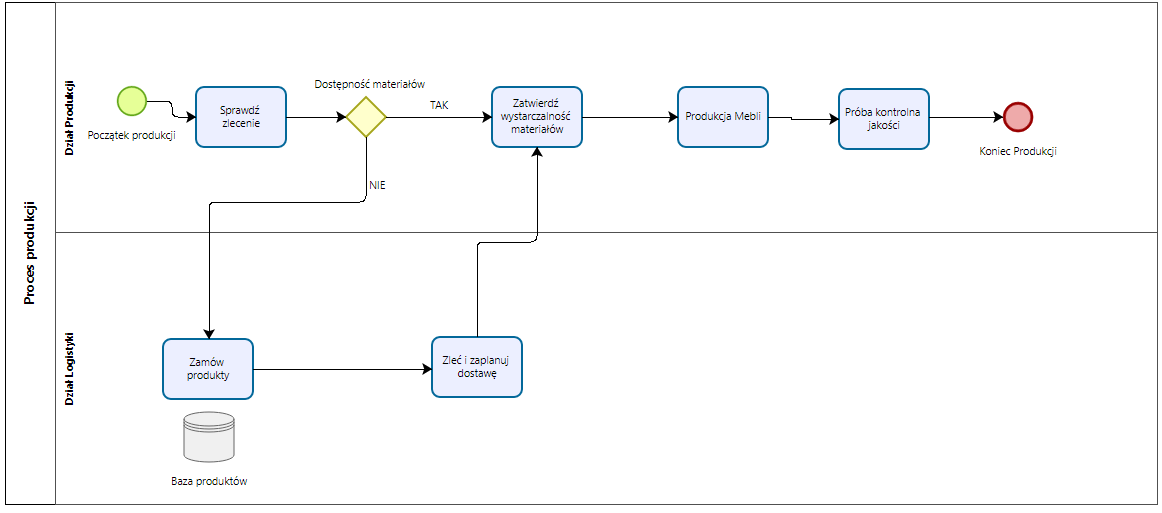
\includegraphics[width=0.9\textwidth]{1.png}\\[0.5cm]
\end{center}
\subsection{Proces montażu}
\begin{center}
    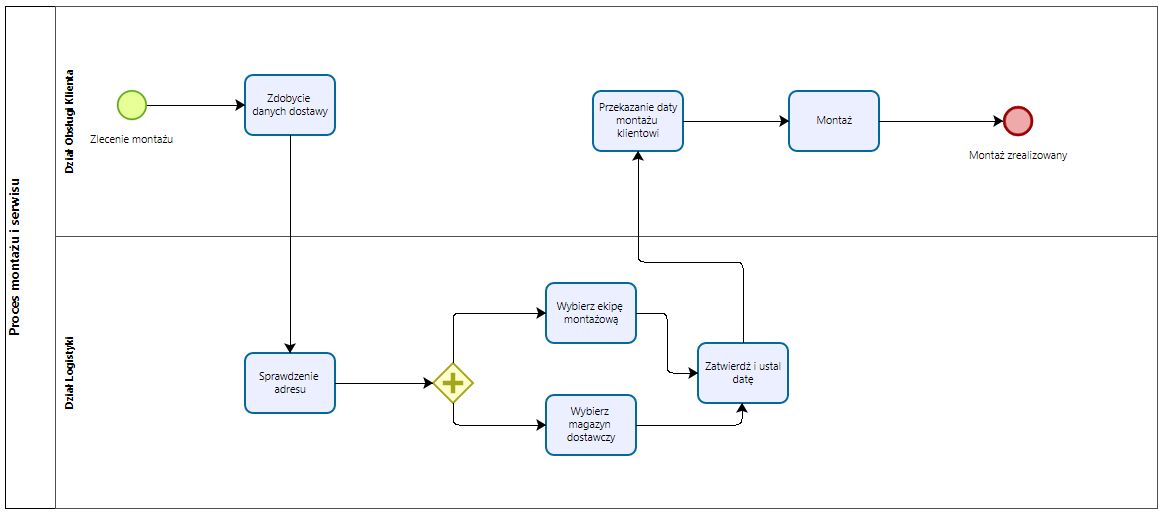
\includegraphics[width=0.9\textwidth]{2.png}\\[0.5cm]
\end{center}
\subsection{Proces zarządzania magazynem}
\begin{center}
    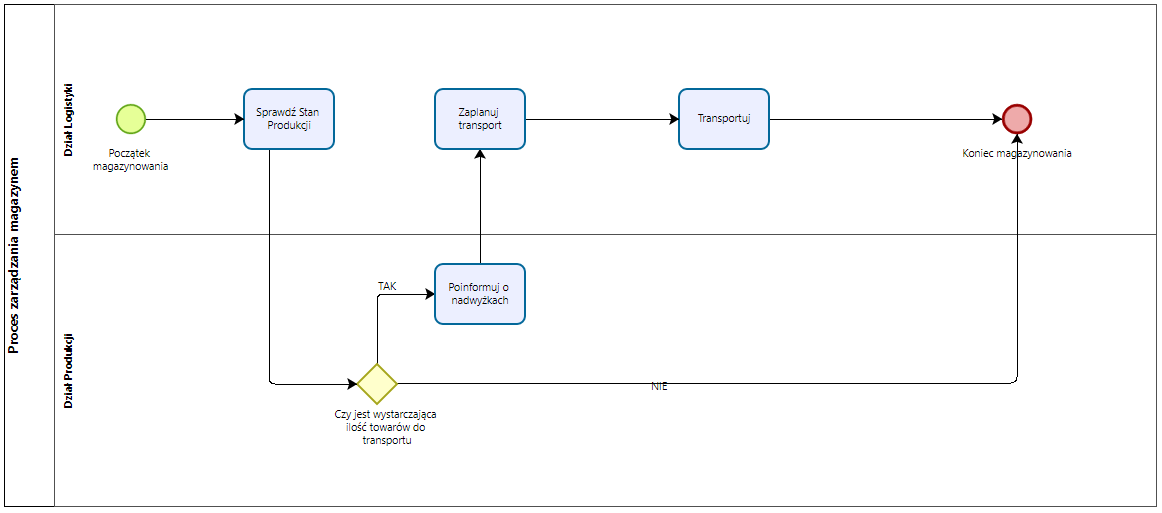
\includegraphics[width=0.9\textwidth]{3.png}\\[0.5cm]
\end{center}

\section{Systemy informatyczne wspierające zarządzanie}
\section{Dane Podstawowe (Master Data)}
\section{Strategia wdrażania systemów}